\documentclass[nohyperref]{article}
\usepackage{microtype}
\usepackage{graphicx}
\usepackage{subfigure}
\usepackage{booktabs} % for professional tables

% hyperref makes hyperlinks in the resulting PDF.
% If your build breaks (sometimes temporarily if a hyperlink spans a page)
% please comment out the following usepackage line and replace
% \usepackage{icml2022} with \usepackage[nohyperref]{icml2022} above.
\usepackage{hyperref}

% Attempt to make hyperref and algorithmic work together better:
\newcommand{\theHalgorithm}{\arabic{algorithm}}

\usepackage[accepted]{icml2022}

% If accepted, instead use the following line for the camera-ready submission:
% \usepackage[accepted]{icml2022}

\usepackage{amsmath}
\usepackage{amssymb}
\usepackage{mathtools}
\usepackage{amsthm}
% if you use cleveref..
\usepackage[capitalize,noabbrev]{cleveref}
\theoremstyle{plain}
\newtheorem{theorem}{Theorem}[section]
\newtheorem{proposition}[theorem]{Proposition}
\newtheorem{lemma}[theorem]{Lemma}
\newtheorem{corollary}[theorem]{Corollary}
\theoremstyle{definition}
\newtheorem{definition}[theorem]{Definition}
\newtheorem{assumption}[theorem]{Assumption}
\theoremstyle{remark}
\newtheorem{remark}[theorem]{Remark}

% Todonotes is useful during development; simply uncomment the next line
%    and comment out the line below the next line to turn off comments
%\usepackage[disable,textsize=tiny]{todonotes}
\usepackage[textsize=tiny]{todonotes}

% The \icmltitle you define below is probably too long as a header.
% Therefore, a short form for the running title is supplied here:
% \icmltitlerunning{WebQA Team 6}

\begin{document}

    \twocolumn[
        \icmltitle{WebQA Data Analysis}

% It is OKAY to include author information, even for blind
% submissions: the style file will automatically remove it for you
% unless you've provided the [accepted] option to the icml2022
% package.

% List of affiliations: The first argument should be a (short)
% identifier you will use later to specify author affiliations
% Academic affiliations should list Department, University, City, Region, Country
% Industry affiliations should list Company, City, Region, Country

% You can specify symbols, otherwise they are numbered in order.
% Ideally, you should not use this facility. Affiliations will be numbered
% in order of appearance and this is the preferred way.
        \icmlsetsymbol{equal}{*}

        \begin{icmlauthorlist}
            \icmlauthor{Haofei Yu}{}
            \icmlauthor{Jiyang Tang}{}
            \icmlauthor{Ruiyi Wang}{}
            \icmlauthor{Ziang Zhou}{}
        \end{icmlauthorlist}

% \icmlaffiliation{cmu}{xxx}

        \icmlkeywords{Machine Learning, ICML}

        \vskip 0.3in
    ]

% this must go after the closing bracket ] following \twocolumn[ ...

% This command actually creates the footnote in the first column
% listing the affiliations and the copyright notice.
% The command takes one argument, which is text to display at the start of the footnote.
% The \icmlEqualContribution command is standard text for equal contribution.
% Remove it (just {}) if you do not need this facility.

%\printAffiliationsAndNotice{}  % leave blank if no need to mention equal contribution
%\printAffiliationsAndNotice{\icmlEqualContribution} % otherwise use the standard text.

%\begin{abstract}
%\end{abstract}


    \section{Statistical Analysis}\label{intro}
    WEBQA \cite{webqa} is a novel and challenging benchmark for multi-modal, multi-hop, open-domain question answering. Generally speaking, this dataset includes 36,766 training samples,  4,966 validation samples, and 7,540 test samples.Based on different annotation standards, the whole dataset can be classified into two types of data: image-based annotated samples and text-based annotated samples. Table \ref{tb:stat1} shows that the image-based annotated samples are 51.24\% of the total number while the text-based annotated samples are 48.76\% of the total number.

    The text-based questions are spread out across a large territory and it makes them hard to find a categorization method that would nicely summarize them into discrete buckets. The linguistic complexity of text-based annotated questions is also greater than that of image-based questions. As a result, tet-based annotated samples are all classified as $\mathit{text}$ and has no fine-grained sub-classes. When it comes to the image-based questions, since these question-answer pairs are more straightforward and easy to answer, the dataset are classified into 6 different types: $\mathit{YesNo}$, $\mathit{choice}$, $\mathit{number}$ , $\mathit{color}$, $\mathit{shape}$ , $\mathit{Other}$.

    More information with regard to question-answer pairs are provided in the WEBQA dataset. The first part of the additional information is the topic of the question-answer pairs. The second part of that is the negative text and image pairs. Concerning topic information, there are 433 different topics in the training dataset and 356 topics in the development dataset. Most of the topics, which include 348 topics, are overlapped between training and development dataset. Only 401 samples in the training dataset own unique topics and only 9 samples in the development dataset have unique topics. Therefore, we can conclude that most topics for the data is shared between training and validation. It means that there is no out-of-distribution problem with regard to training and evaluation.

    Another part of additional information mentioned in the WEBQA dataset is both positive and negative image-based and text-based facts. The negatives in the dataset are hard in a sense that they have large lexical overlap with the question but are not helpful for answering the questions. The positives are carefully checked during the initial annotation process and are ensured that false positives are not included. It is worth noticing that for image-based question-answering pairs, text positives are not provided while for text-based question-answering pairs, image positives are not provided. As a result, we calculate statistical information about positive samples and negative samples separately on image-based question-answering pairs and text-based quetion-answering pairs. Table \ref{tb:stat2} shows how many average positives and negatives belong to each sample in the dataset.

    \begin{table}[t]
        \centering
        \footnotesize
        \begin{tabular}{@{}l@{\hspace{4pt}}r@{\hspace{10pt}}r@{\hspace{10pt}}r@{\hspace{3pt}}r@{\hspace{10pt}}r@{\hspace{6pt}}r@{}}
            WEBQA     & Train(\%) & Dev(\%) & Total(\%) \\
            \toprule
            \# text   & 42.68     & 5.88    & 48.56     \\
            \midrule
            \# YesNo  & 15.56     & 1.98    & 17.54     \\
            \# choice & 8.90      & 1.21    & 10.11     \\
            \# number & 4.45      & 0.61    & 5.06      \\
            \# color  & 3.96      & 0.43    & 4.39      \\
            \# shape  & 1.18      & 0.17    & 1.35      \\
            \# Other  & 11.37     & 1.60    & 12.97     \\
            \midrule
            \midrule
            WEBQA     & \#Train   & \#Dev   & \#Test    \\
            \midrule
            \# sample & 36,766    & 4,966   & 7,540     \\
            \bottomrule
        \end{tabular}
        \caption{Statistical information of WEBQA dataset (Total(\%) column excludes test samples and only considers train and dev samples since the question categorization is not provided in the test dataset).}
        \label{tb:stat1}
        \vspace{-5pt}
    \end{table}


    \begin{table}[t]
        \centering
        \footnotesize
        \begin{tabular}{@{}l@{\hspace{4pt}}r@{\hspace{10pt}}r@{\hspace{10pt}}r@{\hspace{3pt}}r@{\hspace{10pt}}r@{\hspace{6pt}}r@{}}
            Train          & \#Img(+) & \#Img(-) & \#Txt(+) & \#Txt(-) \\
            \toprule
            Image-based QA & 1.44     & 15.85    & 0        & 15.35    \\
            \midrule
            Text-based QA  & 0        & 11.61    & 2.03     & 14.62    \\
            \midrule
            \midrule
            Dev            & \#Img(+) & \#Img(-) & \#Txt(+) & \#Txt(-) \\
            \toprule
            Image-based QA & 1.44     & 15.88    & 0        & 15.29    \\
            \midrule
            Text-based QA  & 0        & 11.78    & 2.04     & 14.63    \\
            \bottomrule
        \end{tabular}
        \caption{Statistical information about both image-based and text-based negatives and positives. Each number in this table represents the average number of text-based and image-based positives and negatives for each sample.}
        \label{tb:stat2}
        \vspace{-5pt}
    \end{table}


    \section{Train-Test Overlap Analysis}
    \citet{qa_overlap} mentions that 60-70\% of test-time answers are also present somewhere in the training sets in widely used open-domain question answering datasets. Moreover, they find that 30\% of
    test-set questions have a near-duplicate paraphrase in their corresponding training sets. In this section, we follow this idea and analyze whether there is answer and question overlap between training dataset and test dataset.

    Mentioned in Section1, since WEBQA has different types of questions and their evaluation metrics are different based on their types, we separately consider their overlap.

    For the first type, including question types of $\mathit{YesNo}$, $\mathit{number}$, $\mathit{color}$, $\mathit{shape}$, WEBQA uses the F1 results calculated from domain keywords and generated tokens as evaluation metrics. For the second type, including question types of $\mathit{choice}$, $\mathit{Other}$ , and $\mathit{text}$, WEBQA uses the recall calculated from test keywords and generated tokens as evaluation metrics.


    \section{Image Fact Aanalysis}

    As mentioned in \cite{webqa}, questions can contain one or two positive image facts and several negative ones.
    The input of the VLP model is the prediction result of a pretrained faster RCNN on such images.
    More specifically, the output of the faster RCNN model's last layer, the bounding
    box coordinates, the object class labels, and the confidence scores are used.

    The negative image facts are obtained using hard negative mining.
    However, \cite{webqa} didn't mention the detailed procedure of this process.
    We obtained more details from the authors.
    During the initial annotation process, each annotator was provided with a set of evidences and
    they selected some of them to create a question that can be answered by these evidences.
    The unselected evidences naturally became negative facts.
    In addition, the authors have a retrieval baseline that selects evidences based on their captions' lexical overlap
    with the question, and the samples that deceived this baseline became additional hard negatives.
    Finally, the authors manually validated these hard negatives to ensure there is no false positive.

    Intuitively, human first read the question and then select which images to use as positive samples based on the
    question content.
    That means the hard negatives must be difficult to be distinguished from each other for the VQA model
    without seeing the question.
    Therefore, we want to verify this assumption by analyzing the image facts without the questions.

    \subsection{Image Embedding Visualization}

    We treat the output of the RCNN model's final layer as the image embeddings, and visualized them with regard to
    positiveness and question type using PCA dimension reduction, as shown in Figure \ref{fig:rcnn_embed_vs_pos_neg} and
    Figure \ref{fig:rcnn_embed_vs_qcate}.

    \begin{figure}[h]
        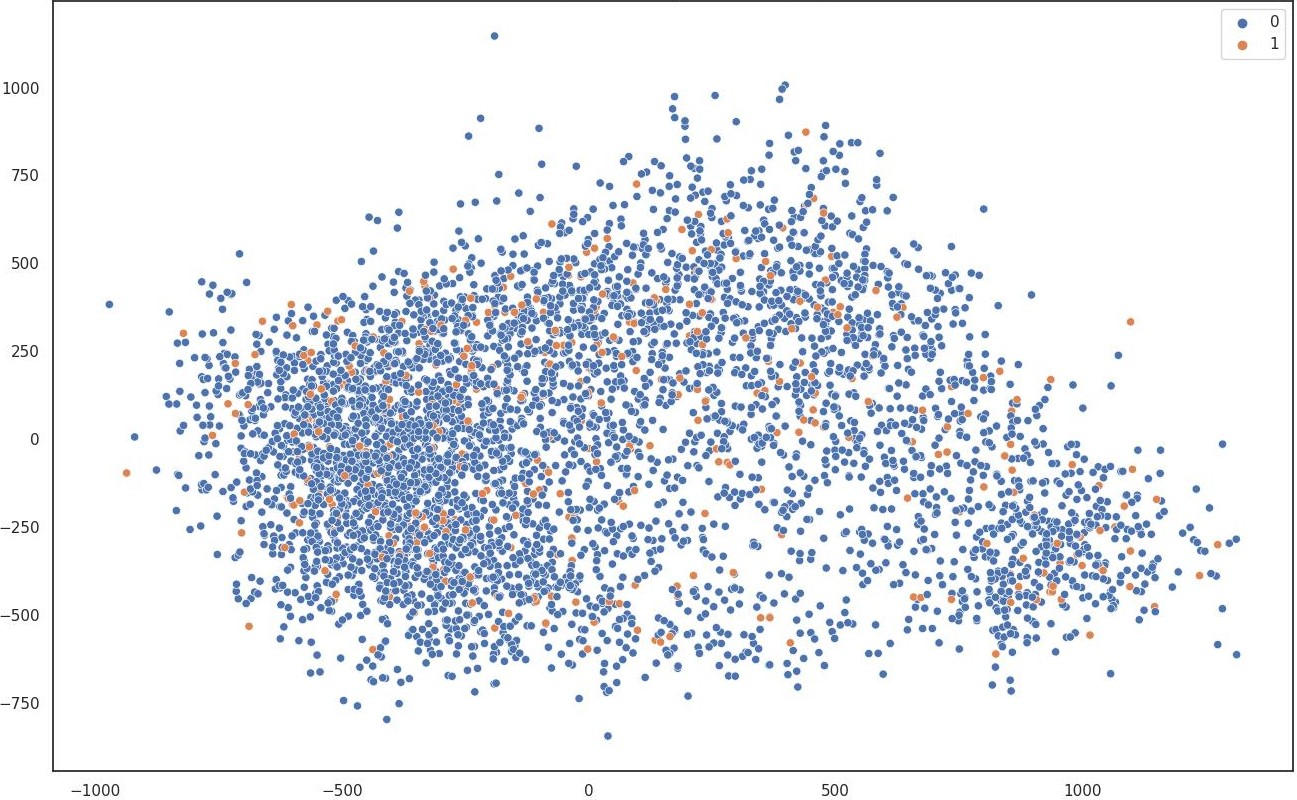
\includegraphics[width=10cm]{rcnn_embed_vs_pos_neg}
        \caption{The PCA of RCNN embeddings vs. positiveness}
        \label{fig:rcnn_embed_vs_pos_neg}
    \end{figure}

    \begin{figure}[h]
        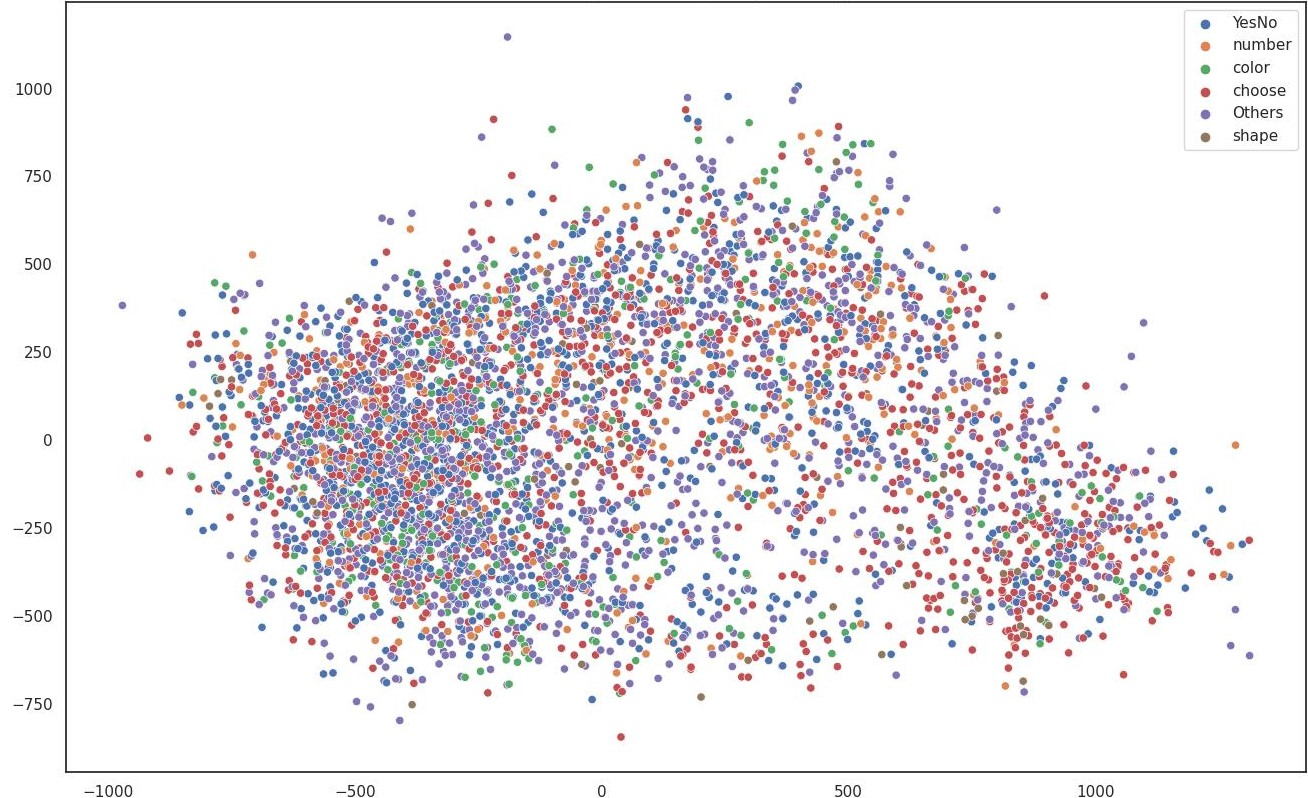
\includegraphics[width=10cm]{rcnn_embed_vs_qcate}
        \caption{The PCA of RCNN embeddings vs. question types}
        \label{fig:rcnn_embed_vs_qcate}
    \end{figure}

    As shown in both figures, there's no apparent pattern or clusters in regard to question types or fact positiveness.
    This gives us a rough impression that the images themselves contain insufficient information to infer their question
    types and fact positiveness.
    However, this doesn't necessarily verify our assumption, because
    \begin{itemize}
        \item there could be some patterns in data that cannot be seen from PCA visualization,
        \item and the RCNN embeddings do not comprehensively represent the images.
    \end{itemize}

    Therefore, to properly verify our assumption, we need to perform some classification experiments on raw image input.

    \begin{table*}[h]
        \centering
        \footnotesize
        \begin{tabular}{lllllll}
            Positiveness   & Positive facts & Negative facts &       &       &        &       \\
            \toprule
            Train          & 2658           & 3673           &       &       &        &       \\
            \midrule
            Test           & 1216           & 1732           &       &       &        &       \\
            \bottomrule
            Question Types & YesNo          & Number         & Color & Shape & Choose & Other \\
            \toprule
            Train          & 369            & 95             & 75    & 28    & 168    & 265   \\
            \midrule
            Test           & 597            & 227            & 160   & 49    & 438    & 529   \\
            \bottomrule
        \end{tabular}
        \caption{Statistics of the image classification subset in terms of positiveness and question types}
        \label{tab:image_classification_subset}
        \vspace{-5pt}
    \end{table*}

    \subsection{Image Classification Experiments}

    We extracted a subset from WebQA that has a balanced number of positive and negative facts.
    See Table \ref{tab:image_classification_subset} for the statistics of the subset.
    In addition, there are 74 question topics in this subset.

    We first need a baseline experiment to prove that our classifier indeed has the capability of
    distinguishing different types of images.
    Therefore, a topic classifier is trained.
    Then, two classifiers are trained, one for predicting question types and the other for predicting fact positiveness.

    We expect the topic classifier to show some classification capability and
    the other two two classifiers to diverge during the training process or to perform badly on the test data.

    The results shown in Table \ref{tab:image_classification_results} indeed meet our expectation.
    \begin{table}[h]
        \centering
        \footnotesize
        \begin{tabular}{lll}
            & Accuracy & F1 Score \\
            \toprule
            Topic Classifier         &          &          \\
            \midrule
            Question Type Classifier &          &          \\
            \midrule
            Positiveness Classifier  &          &          \\
            \bottomrule
        \end{tabular}
        \caption{Image classification experiment results}
        \label{tab:image_classification_results}
        \vspace{-5pt}
    \end{table}

    In conclusion, we believe that the image negatives cannot be distinguished from the positives without seeing the
    questions.


    \section{Future Work}

    \clearpage

    \bibliography{main}
    \bibliographystyle{icml2022}

\end{document}
